\chapter{Data Structure Introduction}

\section*{\Large \textbf{What is Data Structure?}}
Data structures are ways of \textbf{organizing and storing data} so they can be used efficiently. As the name suggests, they involve \hl{organizing data} in memory.

A data structure is \textbf{not a programming language} like \hl{C, C++, Java, or Python}. Instead, it refers to a \textbf{set of algorithms and methods} that can be implemented in any programming language to manage data effectively in memory.

\begin{figure}[!ht]
  \centering
  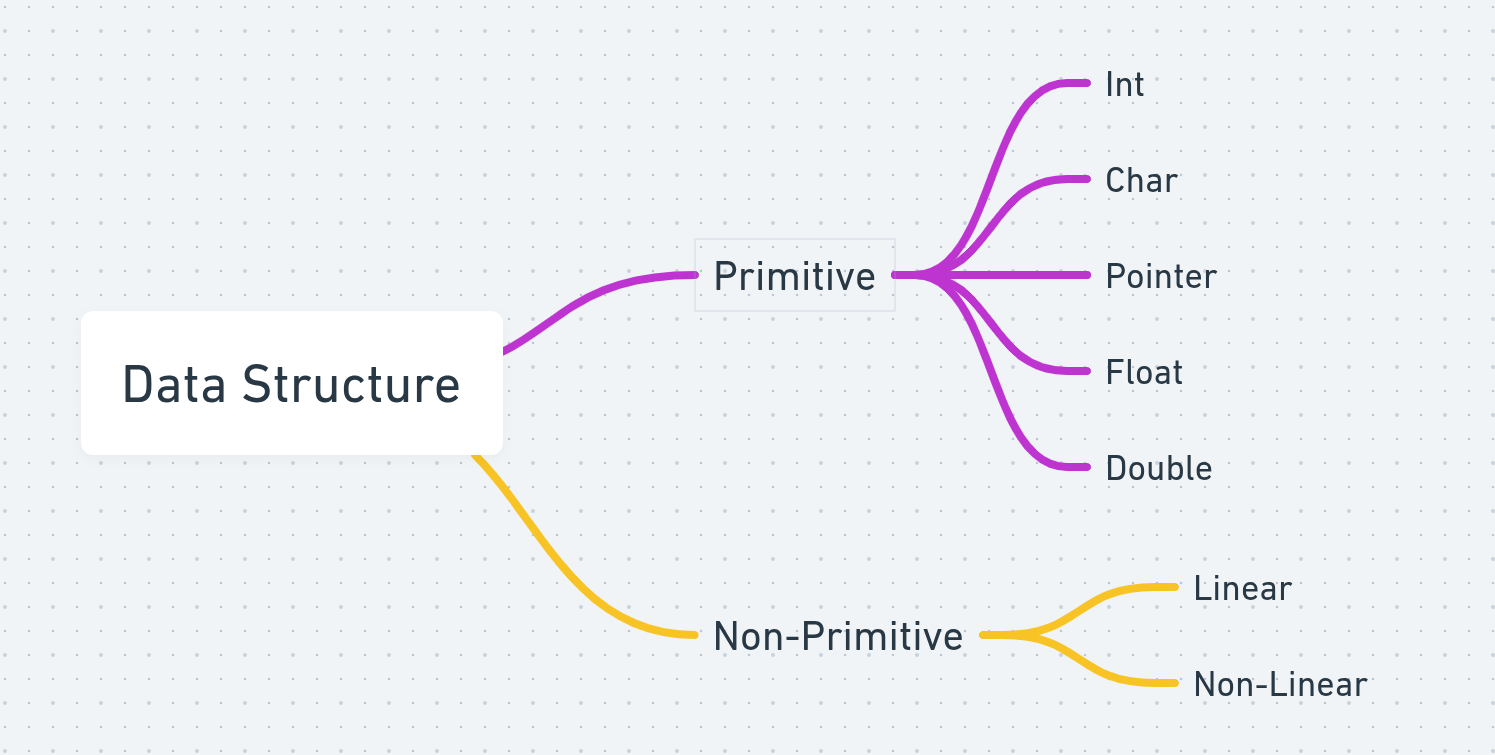
\includegraphics[width=1\textwidth, height=10cm]{images/types.png}
  \caption{Types of Data Structure}
  \label{fig:ds_types}
\end{figure}

\newpage
\section*{\Large \textbf{Linear Data Structure}}
Linear data structures organize elements sequentially, where each element is connected to the next in a \textbf{single level} order. This structure simplifies tasks such as \textbf{traversal, insertion, and deletion}, and includes:

\begin{itemize}
    \item Arrays
    \item Linked Lists
    \item Stacks
    \item Queues
\end{itemize}

\section*{\Large \textbf{Non-Linear Data Structure}}
Non-linear data structures are data structures in which elements are not arranged
sequentially or linearly. Instead, each element can be connected to one or more
elements in a hierarchical or interconnected manner, forming structures like trees
and graphs. These structures are ideal for representing relationships where data
cannot be stored linearly, such as hierarchical relationships (e.g., file systems) or
complex networks (e.g., social networks, maps).
Non-linear data structures organize elements in a \textbf{hierarchical or interconnected manner}, not linearly. These are suitable for representing complex relationships, such as:

\begin{itemize}
    \item \textbf{Trees:} Representing hierarchical data like file systems.
    \item \textbf{Graphs:} Representing networks like social media or maps.
\end{itemize}

\section*{\Large \textbf{Algorithms and Abstract Data Types}}

\begin{figure}[!ht]
  \centering
  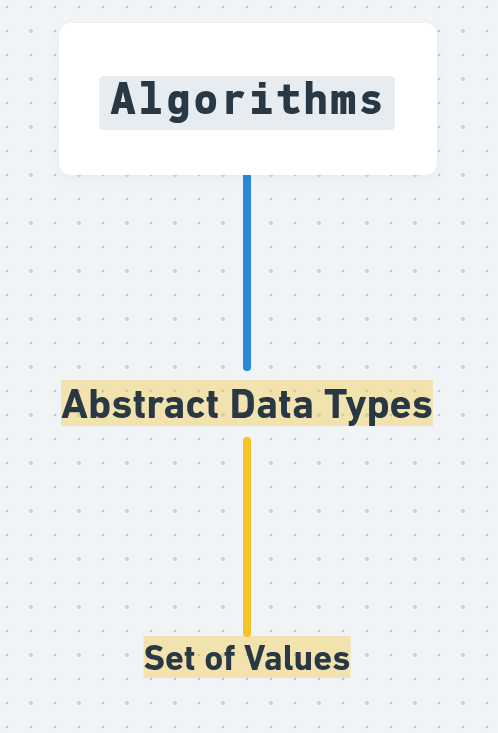
\includegraphics[width=0.6\textwidth, height=10cm]{images/algo.png}
  \caption{Algorithm}
  \label{fig:algo_data}
\end{figure}

\section*{\Large \textbf{Why??..}}
An \textbf{Abstract Data Type (ADT)} is a \textbf{conceptual model} that defines \textbf{what operations can be performed} on data, but \textbf{not how they are implemented}.

\textbf{In simpler terms:}
\begin{itemize}
  \item \textbf{What} the data structure does (its behavior)
  \item \textbf{Not how} it does it (its implementation)
\end{itemize}

\vspace{0.5cm}
\hrule
\vspace{0.5cm}

\subsection*{\normalsize \textbf{Key Characteristics of ADTs:}}
\begin{enumerate}[label=\textbf{\arabic*.}]
  \item \textbf{Abstraction:} Hides implementation details. Users interact with the \textbf{interface}, not internals.
  \item \textbf{Encapsulation:} Bundles \textbf{data and related operations} together.
  \item \textbf{Modularity:} Changes in implementation don’t affect usage.
  \item \textbf{Interface-Based Usage:} Operations like \texttt{insert}, \texttt{delete}, \texttt{search}, etc.
\end{enumerate}

\vspace{0.5cm}
\hrule
\vspace{0.5cm}

\subsection*{\textbf{Examples of Common ADTs:}}
\begin{table}[h!]
\centering
\begin{tabular}{@{}lll@{}}
\toprule
\textbf{ADT} & \textbf{Common Operations} & \textbf{Implemented Using} \\ \midrule
\textbf{List}  & insert, delete, traverse             & Arrays, Linked Lists \\
\textbf{Stack} & push, pop, peek                      & Arrays, Linked Lists \\
\textbf{Queue} & enqueue, dequeue, front, rear        & Arrays, Linked Lists \\
\textbf{Deque} & insertFront, insertRear, deleteFront, deleteRear & Arrays, Linked Lists \\
\bottomrule
\end{tabular}
\caption{Examples of Common Abstract Data Types}
\end{table}

\newpage
\section*{\Large \textbf{Basic Terminology}}

\subsection*{\textbf{1. What is Data?}}
\textbf{Data} refers to raw facts and figures that have no meaning by themselves but can be processed to gain useful information. These could be \textbf{numbers, text, images, audio, etc}.

\subsection*{\textbf{2. What is Record?}}
A \textbf{record} is a collection of \textbf{related data items or fields} that describe one entity or object. It often combines multiple \textbf{attributes}.

\subsection*{\textbf{3. What is File?}}
A \textbf{file} is a collection of related records stored together. It is a \textbf{unit of data storage} and often represents a complete dataset.

\subsection*{\textbf{4. What is an Attribute?}}
An \textbf{attribute} is a \textbf{characteristic or property} of an entity, describing one aspect of it.

\subsection*{\textbf{5. What is Entity?}}
An \textbf{entity} is a real-world \textbf{object or concept} with data stored about it. It’s typically represented as a \textbf{record}.

\section*{\Large \textbf{Need for Data Structures}}
Efficient data handling is \textbf{crucial} in computer science. As software grows in complexity, \textbf{organization and management of data} becomes essential. That’s where \textbf{data structures} help.

\subsection*{\textbf{1. Efficient Data Access and Processing}}
They enable \textbf{fast access, retrieval, and updates} — e.g., \texttt{arrays} allow direct indexing, \texttt{hash tables} provide constant-time lookup.

\subsection*{\textbf{2. Code Optimization}}
Choosing the right structure improves \textbf{time and space complexity}, leading to more \textbf{efficient code}.

\subsection*{\textbf{3. Data Organization}}
Logical arrangement (e.g., \texttt{trees}, \texttt{graphs}) simplifies representation of \textbf{relationships and hierarchy}.

\subsection*{\textbf{4. Reusability and Modularity}}
Abstract data structures allow for \textbf{modular design}, enhancing reuse across applications.

\subsection*{\textbf{5. Real-World Problem Solving}}
Applications like \textbf{search engines, databases, and social networks} rely on well-structured data.

\subsection*{\textbf{6. Memory Management}}
Structures like \texttt{linked lists} or \texttt{trees} support \textbf{dynamic memory allocation} and efficient usage.

\subsection*{\textbf{7. Algorithm Design}}
Most \textbf{algorithms} are designed around a \textbf{specific data structure} — making DSA foundational.

\subsection*{\textbf{8. Scalability}}
\textbf{Scalable structures} ensure performance doesn’t degrade with increased data.

\vspace{0.5cm}
\hrule
\vspace{0.5cm}

\section*{\Large \textbf{Advantages of Data Structures}}
\begin{itemize}
    \item \textbf{Improved Performance:} Optimized code runs faster.
    \item \textbf{Efficient Memory Usage:} Reduces memory wastage.
    \item \textbf{Reusability:} Use across multiple programs.
    \item \textbf{Maintainability:} Easier debugging and management.
    \item \textbf{Enhanced Productivity:} Simplifies complex logic.
    \item \textbf{Foundation of Algorithm Development:} Core of problem-solving.
    \item \textbf{Support for Complex Computations:} Trees, graphs enable solving advanced problems.
\end{itemize}
